\documentclass{standalone}
\usepackage{pgfplots}
\begin{document}
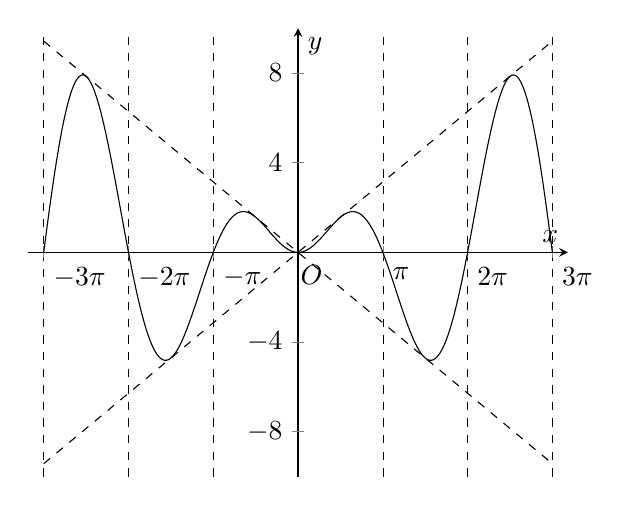
\begin{tikzpicture}
\begin{axis}
[
ymin=-10,ymax=10,
xmin=-10,xmax=10,
xtick=\empty,
ytick=\empty,
extra x ticks={-9.42478, -6.28319, -3.14159, 3.14159, 6.28319, 9.42478},
extra x tick labels={$-3\pi$, $-2\pi$, $-\pi$, $\pi$, $2\pi$, $3\pi$},
extra y ticks={-8, -4, 4, 8},
extra y tick labels={$-8$, $-4$, $4$, $8$},
every extra x tick/.style={
    xticklabel style={anchor=north west},
    grid=major,
    major grid style={very thin,dashed,black}
},
axis lines = center,
xlabel=$x$,ylabel=$y$,
samples=200,
]
\addplot [black, domain=-9.42478:9.42478, samples=400] {x*sin(deg(x))};
\addplot [black, dashed, domain=-9.42478:9.42478] {x};
\addplot [black, dashed, domain=-9.42478:9.42478] {-x};
\node at (axis cs:0.5, -1) {$O$} ;
\end{axis}
\end{tikzpicture}
\end{document}
